\documentclass{beamer}
\usepackage{array}
\usepackage{graphicx}
\usepackage{xcolor}
\usepackage{graphicx}
\usepackage{amsmath}

\usetheme{Madrid}

% Suppress the navigation bar and remove name and date from slides
\setbeamertemplate{navigation symbols}{}
\setbeamertemplate{footline}{}  % Removes the footer line with the author and date
\setbeamertemplate{headline}{}  % Removes the header line

% Title page details
\title{Conversational Used Car Price Predictor}
\subtitle{CS702 - Computing Lab}
\author{ABHIJITH C \and ANAND M K}
\institute{Department of Computer Science and Engineering \\ NITK Surathkal}
\date{}  % No date on title slide

\begin{document}

% Title page
\begin{frame}[t]
    \titlepage
\end{frame}

\begin{frame}[t]{Introduction}
    \begin{itemize}
        \item This project focuses on developing a \textbf{Conversational Used Car Price Predictor}, integrating a chatbot interface with a machine learning model.
\item The chatbot will collect necessary car details (brand, model, year, mileage, etc.) step by step through an interactive and engaging interface.
        \item A machine learning model will use the gathered data to predict the price of the used car, ensuring accurate and reliable predictions.
        \item The chatbot also handles additional queries, such as explaining how the price was calculated or what factors affect the car’s value.
    \end{itemize}
\end{frame}


\begin{frame}{System Architecture}'
    \centering
   	 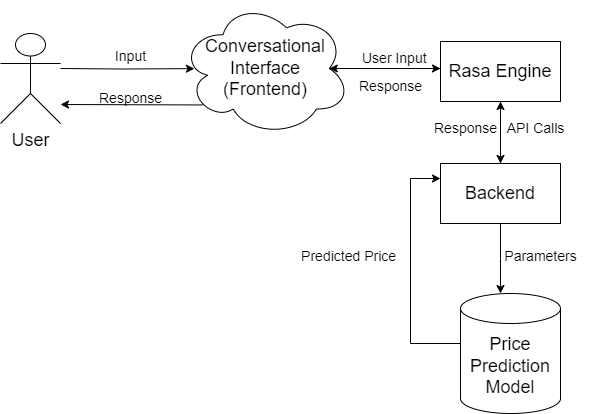
\includegraphics[width=0.8\textwidth]{Midsem.drawio.png}
\end{frame}

\begin{frame}{System Flow Explanation}
    \begin{itemize}
        \item The user interacts with the system via a chat interface in the frontend, initiating a conversation to predict the price of their used car.
        \item The user inputs (car details such as make, model, year, mileage, etc.) are processed by the \textbf{Rasa Engine}, which handles NLP and conversation management.
        \item The Rasa Engine extracts relevant parameters from the conversation and sends them to the backend, where the \textbf{Price Prediction Model} calculates the car's estimated price based on the input features.
        \item \textbf{SHAP} (SHapley Additive exPlanations) is applied to explain the contribution of each feature (e.g., mileage, car age, etc.) to the final price prediction, identifying the most impactful factor.
        \item The backend returns both the predicted price and the explanation of the most significant contributing factor, which are displayed to the user through the chat interface.
    \end{itemize}
\end{frame}


\begin{frame}{Implementation of Random Forest for Price Prediction}
    \begin{itemize}
        \item \textbf{Dataset and Preprocessing:}
        \begin{itemize}
            \item Dataset sourced from Kaggle: \texttt{cardekho\_dataset} in 2023.
            \item Categorical features (\texttt{fuel\_type}, \texttt{transmission\_type}, \texttt{brand}, \texttt{model}) encoded using One-Hot Encoding.
        \end{itemize}
        
        \item \textbf{Model Building:}
        \begin{itemize}
            \item \textbf{Random Forest Regressor} used for price prediction.
            \item Hyperparameters tuned using \texttt{RandomizedSearchCV} for optimal performance:
            \begin{itemize}
                \item \texttt{n\_estimators}: Number of trees in the forest.
                \item \texttt{max\_depth}: Maximum depth of each tree, controlling tree complexity.
                \item \texttt{min\_samples\_split}: Minimum samples required to split an internal node.
                \item \texttt{min\_samples\_leaf}: Minimum samples required to be at a leaf node.
            \end{itemize}
        \end{itemize}
        
        \item \textbf{Model Evaluation:}
        \begin{itemize}
            \item \textbf{R² Score:} 0.93, meaning the model can predict 93\% of the changes in car prices based on the provided features, indicating a high level of accuracy.
            \item \textbf{Mean Absolute Error (MAE):} 6089.98, representing the average deviation from actual prices.
        \end{itemize}
    \end{itemize}
\end{frame}




\begin{frame}{Finding the Most Influential Feature using SHAP Values}
    \begin{itemize}
        \item The input data is first preprocessed using the same steps as during model training, ensuring consistency in feature transformations.
        \item SHAP (SHapley Additive exPlanations) values are then calculated to explain the contribution of each feature to the model’s predicted output.
        \item The SHAP values quantify the impact of each feature, allowing us to identify which feature has the maximum influence on the predicted price.
        \item The feature with the highest SHAP value is considered the most influential in determining the car's price.
        \item The percentage contribution of this most influential feature is computed by dividing its SHAP value by the predicted price, giving an understanding of its relative importance.
    \end{itemize}
\end{frame}





\begin{frame}{Backend API Creation}
    \begin{itemize}
        \item \textbf{Framework Used:} Flask
        \begin{itemize}
            \item A lightweight web framework for Python, used to create web applications.
        \end{itemize}
        
        \item \textbf{Endpoints:}
        \begin{itemize}
            \item \texttt{/predict\_price}: 
            \begin{itemize}
                \item Accepts car attributes as query parameters.
                \item Returns the predicted selling price of the car.
            \end{itemize}
            \item \texttt{/max\_contribution}: 
            \begin{itemize}
                \item Accepts the same car attributes as query parameters.
                \item Returns the highest contributing feature to the predicted price and its percentage contribution.
            \end{itemize}
        \end{itemize}
        
        \item \textbf{Input Handling:}
        \begin{itemize}
            \item Retrieves input data via query parameters (GET API).
        \end{itemize}
        
        \item \textbf{Response Format:}
        \begin{itemize}
            \item Outputs predictions and contributions as JSON, facilitating easy integration with frontend applications.
        \end{itemize}
    \end{itemize}
\end{frame}


\begin{frame}{Chatbot Development using Rasa}
    \begin{itemize}
        \item Rasa is an open-source framework for building conversational AI applications, supporting both rule-based and machine-learning-driven chatbots.
    \end{itemize}
    
    \begin{block}{Rasa Core Workflow}
        \begin{enumerate}
            \item User input is processed by the NLU module to identify \textbf{intents} and \textbf{entities}.
            \item The extracted information is passed to the \textbf{dialogue manager}, which uses a set of rules to decide the next action.
            \item The bot executes the selected action, such as providing a response or performing a backend operation.
            \item The conversation state is updated to ensure continuity in subsequent interactions.
        \end{enumerate}
    \end{block}
\end{frame}


\begin{frame}{Intents Overview}
    \begin{itemize}
        \item \textbf{What is an Intent?} \\
        An intent represents the user's goal or purpose behind a specific input. It helps the chatbot understand the context of the conversation and respond accordingly.
        
        \item \textbf{Greet}: Recognizes user greetings and initiates the conversation.
        \item \textbf{Goodbye}: Handles farewell phrases to end the conversation.
        \item \textbf{Affirm}: Detects user confirmation or agreement.
        \item \textbf{Deny}: Identifies when the user disagrees or negates a statement.
        \item \textbf{Bot Challenge}: Handles questions about the chatbot's identity.
        \item \textbf{Inform}: Collects user-provided details about the car (e.g., brand, model, mileage).
        \item \textbf{Stop}: Ends the conversation when the user requests it.
        \item \textbf{Ask SHAP}: Explains factors affecting car price prediction using SHAP values.
        \item \textbf{Ask Mileage}: Explains the meaning and impact of mileage on car pricing.
    \end{itemize}
\end{frame}


\begin{frame}
	\frametitle{Entities in NLU}
	
	\begin{itemize}
		\item
Entities refer to the specific pieces of information that the chatbot extracts from the user's input. These are usually key elements that represent important details for processing the user's request, like car attributes in this case.
		
		\item \textbf{brand} - represents the car brand (e.g., Toyota, Ford, etc.)
		\item \textbf{model} - represents the car model (e.g., Fortuner, Swift, etc.)
		\item \textbf{mileage} - represents the car's mileage (e.g., 15 km/l)
		\item \textbf{km\_driven} - represents the distance the car has been driven (e.g., 10000 km)
		\item \textbf{fuel\_type} - represents the type of fuel the car uses (e.g., petrol, diesel)
		\item \textbf{transmission\_type} - represents the transmission type of the car (e.g., manual, automatic)
		\item \textbf{engine} - represents the engine capacity of the car (e.g., 1500 cc)
		\item \textbf{max\_power} - represents the car's maximum power (e.g., 150 bhp)
		\item \textbf{seats} - represents the seating capacity of the car (e.g., 5 seats)
		\item \textbf{year\_of\_manufacture} - represents the car's year of manufacture
	\end{itemize}
	
\end{frame}


	
\begin{frame}
	\frametitle{Entity Extraction Using Regular Expressions}

	Regular expressions (\textbf{regex}) are a powerful tool used in the chatbot for extracting specific entities from user inputs. They enable precise matching of patterns in text, making it possible to capture key details efficiently. Below are the regex patterns used for extracting entities along with examples:

	\begin{itemize}
		
		\item \textbf{Mileage:} Identifies the car's fuel efficiency, typically followed by units like \texttt{km/l}.
		\\ \textbf{Regex Pattern:} \texttt{\textbackslash b\textbackslash d\{1,2\}\textbackslash b(?=\textbackslash s*(kmpl|km/l|km per liter)\textbackslash b)}
		\\ \textbf{Example:} \texttt{18 km/l}
		
		\item \textbf{Engine Capacity (\texttt{engine}):} Extracts the engine size in cubic centimeters (\texttt{cc}).
		\\ \textbf{Regex Pattern:} \texttt{\textbackslash b(\textbackslash d\{3,4\})\textbackslash s?cc\textbackslash b}
		\\ \textbf{Example:} \texttt{1500 cc}
	\end{itemize}
\end{frame}

\begin{frame}
	\frametitle{Entity Extraction Using Lookup Tables}

	Lookup tables are used to extract entities by matching user inputs against predefined lists of possible values. This approach is particularly effective for entities such as \texttt{brand} and \texttt{model}, ensuring accurate recognition of user-provided information.

	\begin{itemize}
		\item \textbf{Brand:} The \texttt{brand} entity is extracted using a lookup table containing names of car manufacturers.
		\\ \textbf{Examples:}
		\begin{itemize}
			\item \texttt{Maruti}
			\item \texttt{Hyundai}
		\end{itemize}
		
		\item \textbf{Model:} The \texttt{model} entity is extracted using a lookup table with car model names.
		\\ \textbf{Examples:}
		\begin{itemize}
			\item \texttt{Alto}
			\item \texttt{Swift}
		\end{itemize}
	\end{itemize}
\end{frame}


\begin{frame}
	\frametitle{Slots and Forms in Rasa}

	Slots and forms are key components of Rasa that manage the flow of conversation and the collection of necessary information.

	\begin{itemize}
		\item \textbf{Slots:} Store values collected during the conversation. They track important information, such as car details.
		\\ \textbf{Examples:}
		\begin{itemize}
			\item \texttt{brand} - Stores the car's brand (e.g., \texttt{Maruti}, \texttt{Hyundai})
			\item \texttt{model} - Stores the car model (e.g., \texttt{Alto}, \texttt{i20})
			\item \texttt{km\_driven} - Stores the number of kilometers driven (e.g., \texttt{50000 km})
		\end{itemize}

		\item \textbf{Forms:} Guide the user through a sequence of questions to collect all the necessary information.
	Forms ensure the chatbot collects all the required details before proceeding with a task.
	\end{itemize}


\end{frame}

\begin{frame}
	\frametitle{Form Responses in Rasa}

	Form responses are predefined messages that guide the user to provide specific information for the chatbot.

	\begin{itemize}
		\item \textbf{utter\_ask\_brand:} Asks for the car's brand.
		\\ \textbf{Example:} "Great! Let's start with the basics. What’s the brand of your car?"
		\\ This helps gather brand details (e.g., "Hyundai", "Ford").
		
		\item \textbf{utter\_ask\_model:} Asks for the car's model.
		\\ \textbf{Example:} "Got it. And what’s the model?"
		\\ This helps collect the model (e.g., "Creta", "Figo").
	\end{itemize}
\end{frame}



\begin{frame}{Form Validation}
	\begin{itemize}
		\item \textbf{Brand \& Model}: Fuzzy matching with predefined lists of car brands/models.
		\item \textbf{Numeric Slots}: Checks ranges for km driven, mileage, engine capacity, max power, seats, and year of manufacture.
		\item \textbf{Fuel Type \& Transmission}: Validates against allowed values like \texttt{petrol}, \texttt{diesel}, \texttt{automatic}, etc.
	\end{itemize}
\end{frame}


\begin{frame}
	\frametitle{Custom Actions to Call APIs}

	\textbf{Action-PredictCarPrice:}
	\begin{itemize}
		\item Extracts car details from slots (e.g., brand, model, mileage).
		\item Sends GET request to \texttt{predict\_price} API.
		\item Displays predicted car price if successful.
		\item Displays error message if the request fails.
	\end{itemize}

	\textbf{Action-MaxContribution:}
	\begin{itemize}
		\item Checks if all car details are provided.
		\item Sends data to \texttt{max\_contribution} API to identify the most impactful feature on the car price.
		\item Displays the highest contributing feature and its percentage.
		\item Displays error message if the request fails.
	\end{itemize}
\end{frame}

\begin{frame}
	\frametitle{Rules for Conversation Flow}

	\textbf{Overview:} \\
	The rules define how the chatbot responds to various user inputs, ensuring a smooth conversation flow. They specify sequences of actions triggered by user intents, conditions, or situations. 
	
\textbf{Say 'I am a bot' anytime the user challenges:}
	\begin{itemize}
		\item Triggered when the user asks about the bot's identity.
		\item Example: "Who are you?"
		\item Response: "I am a bot."
	\end{itemize}
	
	\textbf{Initial Greet:}
	\begin{itemize}
		\item Triggered when the user greets the bot.
		\item Example: "Hello!"
		\item Response: "Hi! How can I assist you today?"
	\end{itemize}

	\textbf{Activate Car Details Form:}
	\begin{itemize}
		\item Triggered when the user mentions car details.
		\item Example: "I want to know the price of my car."
		\item Response: Asks for car details like brand, model, mileage, etc.
	\end{itemize}
\end{frame}

\begin{frame}
	\frametitle{Handling General Queries}

	\textbf{Overview:} \\
This section highlights how the chatbot responds to general queries related to car specifications and pricing factors.

	\textbf{Ask Mileage:}
	\begin{itemize}
		\item Examples:
		\begin{itemize}
			\item "What is mileage?"
			\item "How is mileage measured?"
		\end{itemize}
		\item Response: "Mileage refers to how far a vehicle can travel on a unit of fuel, typically measured in kilometers per liter (km/l) or miles per gallon (mpg). It can be affected by factors like engine size and driving habits."
	\end{itemize}

	\textbf{Ask Value Calculation:}
	\begin{itemize}
		\item Examples:
		\begin{itemize}
			\item "How is the value of a car calculated?"
			\item "What factors determine a car's price?"
		\end{itemize}
		\item Response: "The value of a car is calculated using a machine learning model trained on real-time data, considering parameters such as the car's age, mileage, engine capacity, brand, model and fuel type."
	\end{itemize}

\end{frame}


\begin{frame}{Rasa Telegram Integration}
    Telegram serves as the frontend for the car price prediction chatbot, offering a user-friendly and easy-to-use platform for users to interact with the system.

    \textbf{Steps for Integration:}
    \begin{itemize}
        \item \textbf{Create Telegram Bot:}  
        A bot is created using Telegram's \texttt{@BotFather}, which provides a unique token to authenticate and connect the bot to external platforms like Rasa.
        
        \item \textbf{Configuration in Rasa:}  
        Telegram's bot details (access token and bot name) are added to Rasa's configuration. This enables Rasa to communicate with Telegram.
        
        \item \textbf{Webhook Setup:}  
        A webhook URL is configured to allow Telegram to forward incoming user messages to the Rasa server for processing.
        
        \item \textbf{Message Flow:}  
        \begin{itemize}
            \item User sends a message to the Telegram bot.
            \item Telegram forwards the message to Rasa.
            \item Rasa processes the message, determines the intent, and generates an appropriate response.
            \item The response is sent back to Telegram, which delivers it to the user.
        \end{itemize}
    \end{itemize}
\end{frame}

\begin{frame}
\frametitle{Conclusion}

\begin{itemize}
    \item \textbf{Chatbot using Rasa}: The chatbot enables conversational interaction, allowing users to input car details and receive price predictions.

    \item \textbf{Price Prediction using Machine Learning}: A RandomForestRegressor model predicts car prices based on user-provided details.
    \item \textbf{SHAP for Identifying Influential Features}: SHAP values help explain the most influential features driving car price predictions.
    \item \textbf{Backend API using Flask}: Flask processes user input and serves predictions along with SHAP-based explanations.
    \item \textbf{Frontend using Telegram}: Telegram serves as the platform for user interaction, providing a user-friendly interface for car price predictions.
\end{itemize}

\end{frame}


\begin{frame}
\frametitle{Sample Chat Screenshots (Part 1)}

\begin{figure}[h!]
    \begin{minipage}{0.45\textwidth}
        \centering
        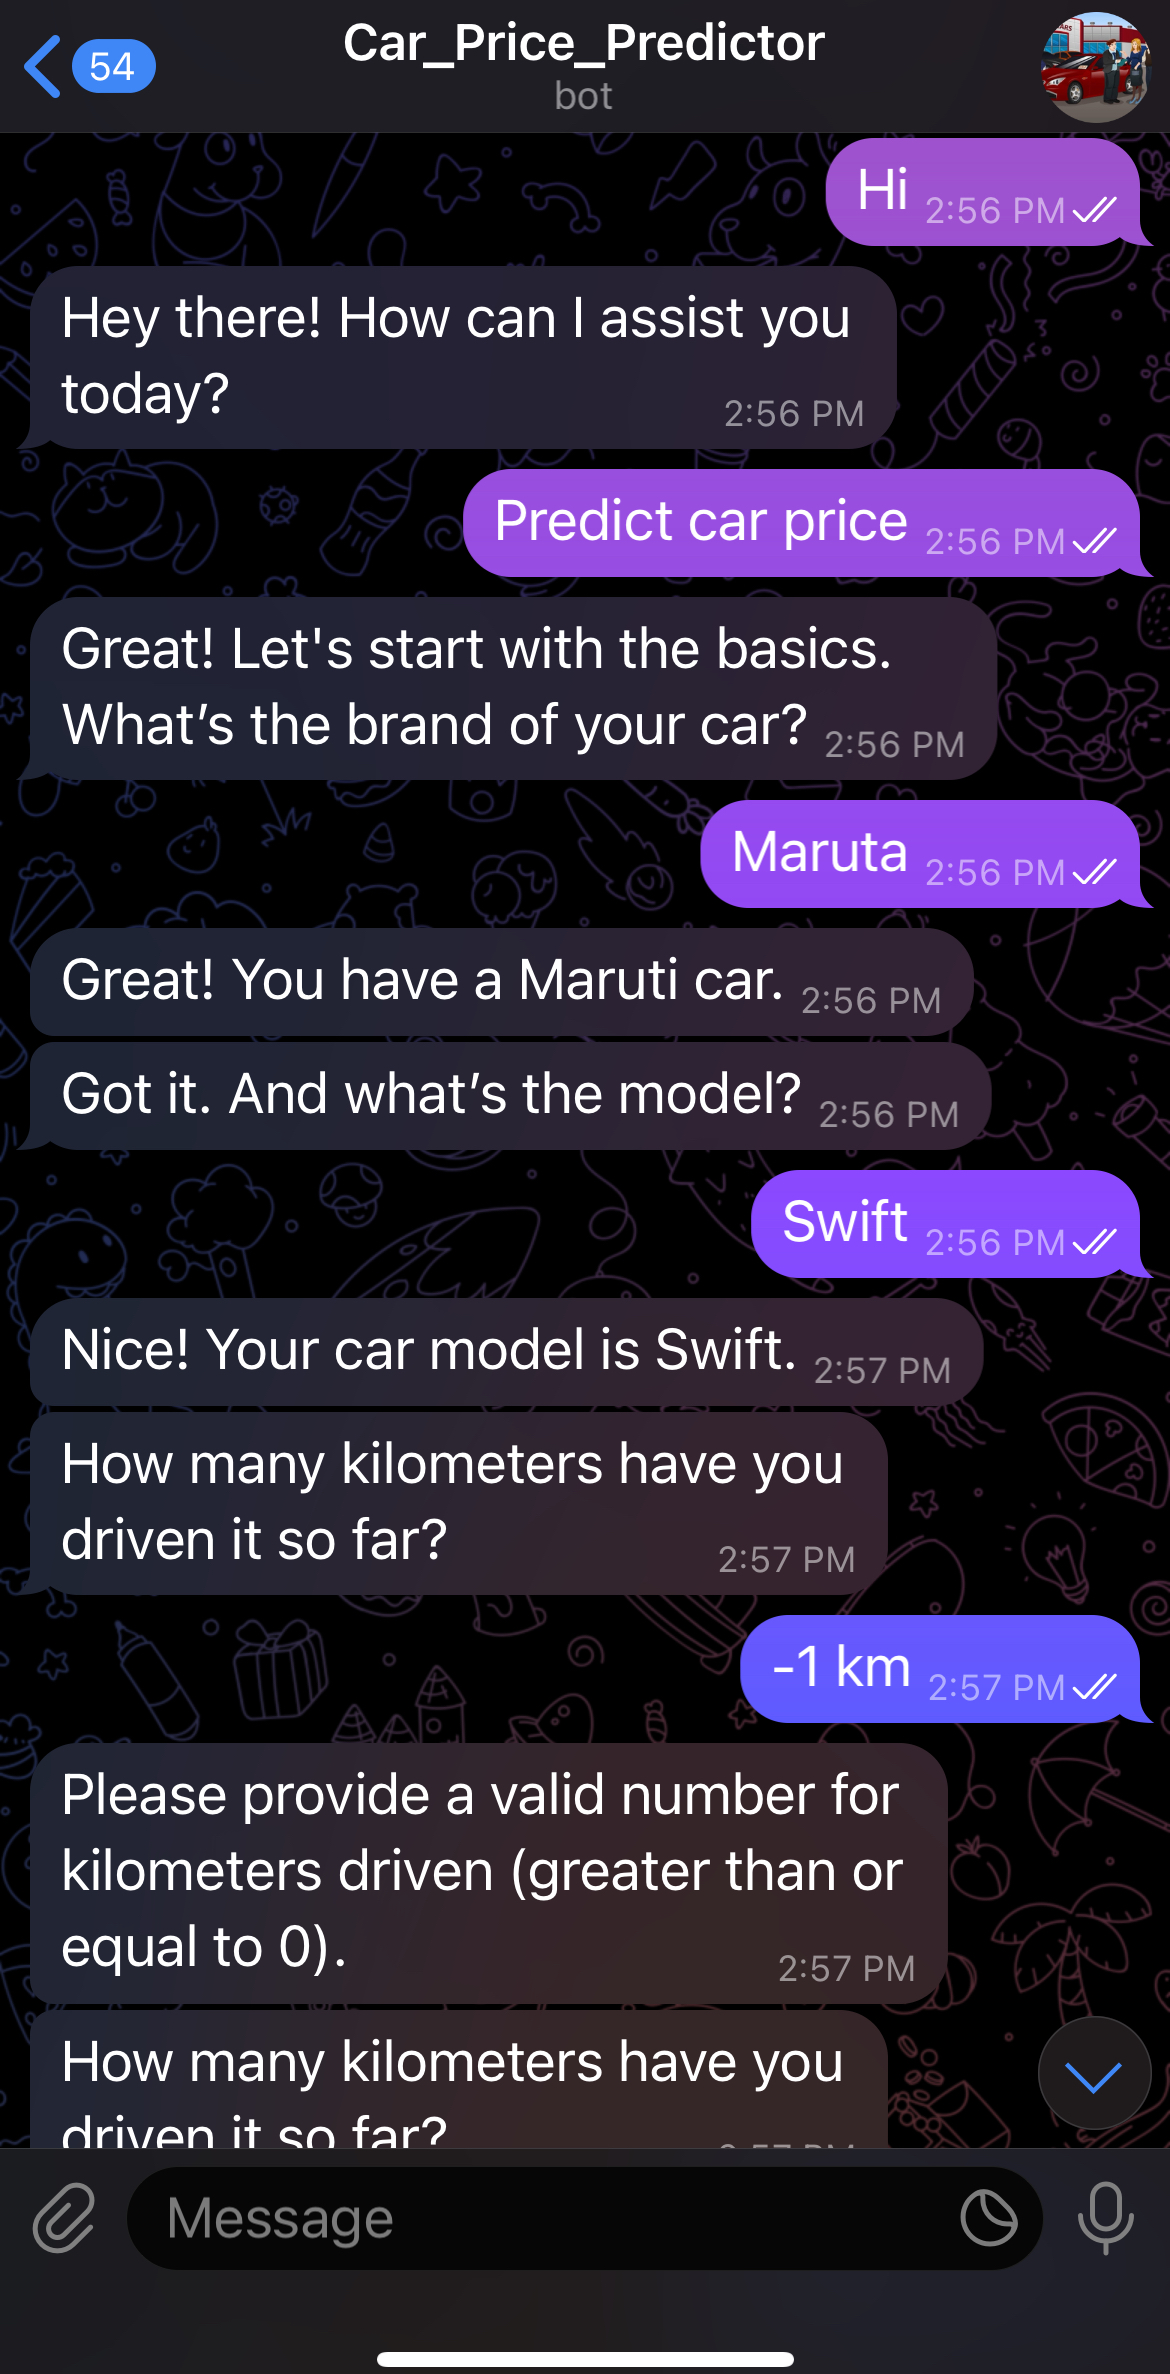
\includegraphics[width=0.8\textwidth]{1.jpg}
        \caption{Chat Flow Step 1: User requests car price prediction.}
        \label{fig:step1}
    \end{minipage}%
    \hspace{0.05\textwidth} % Add space between the images
    \begin{minipage}{0.45\textwidth}
        \centering
        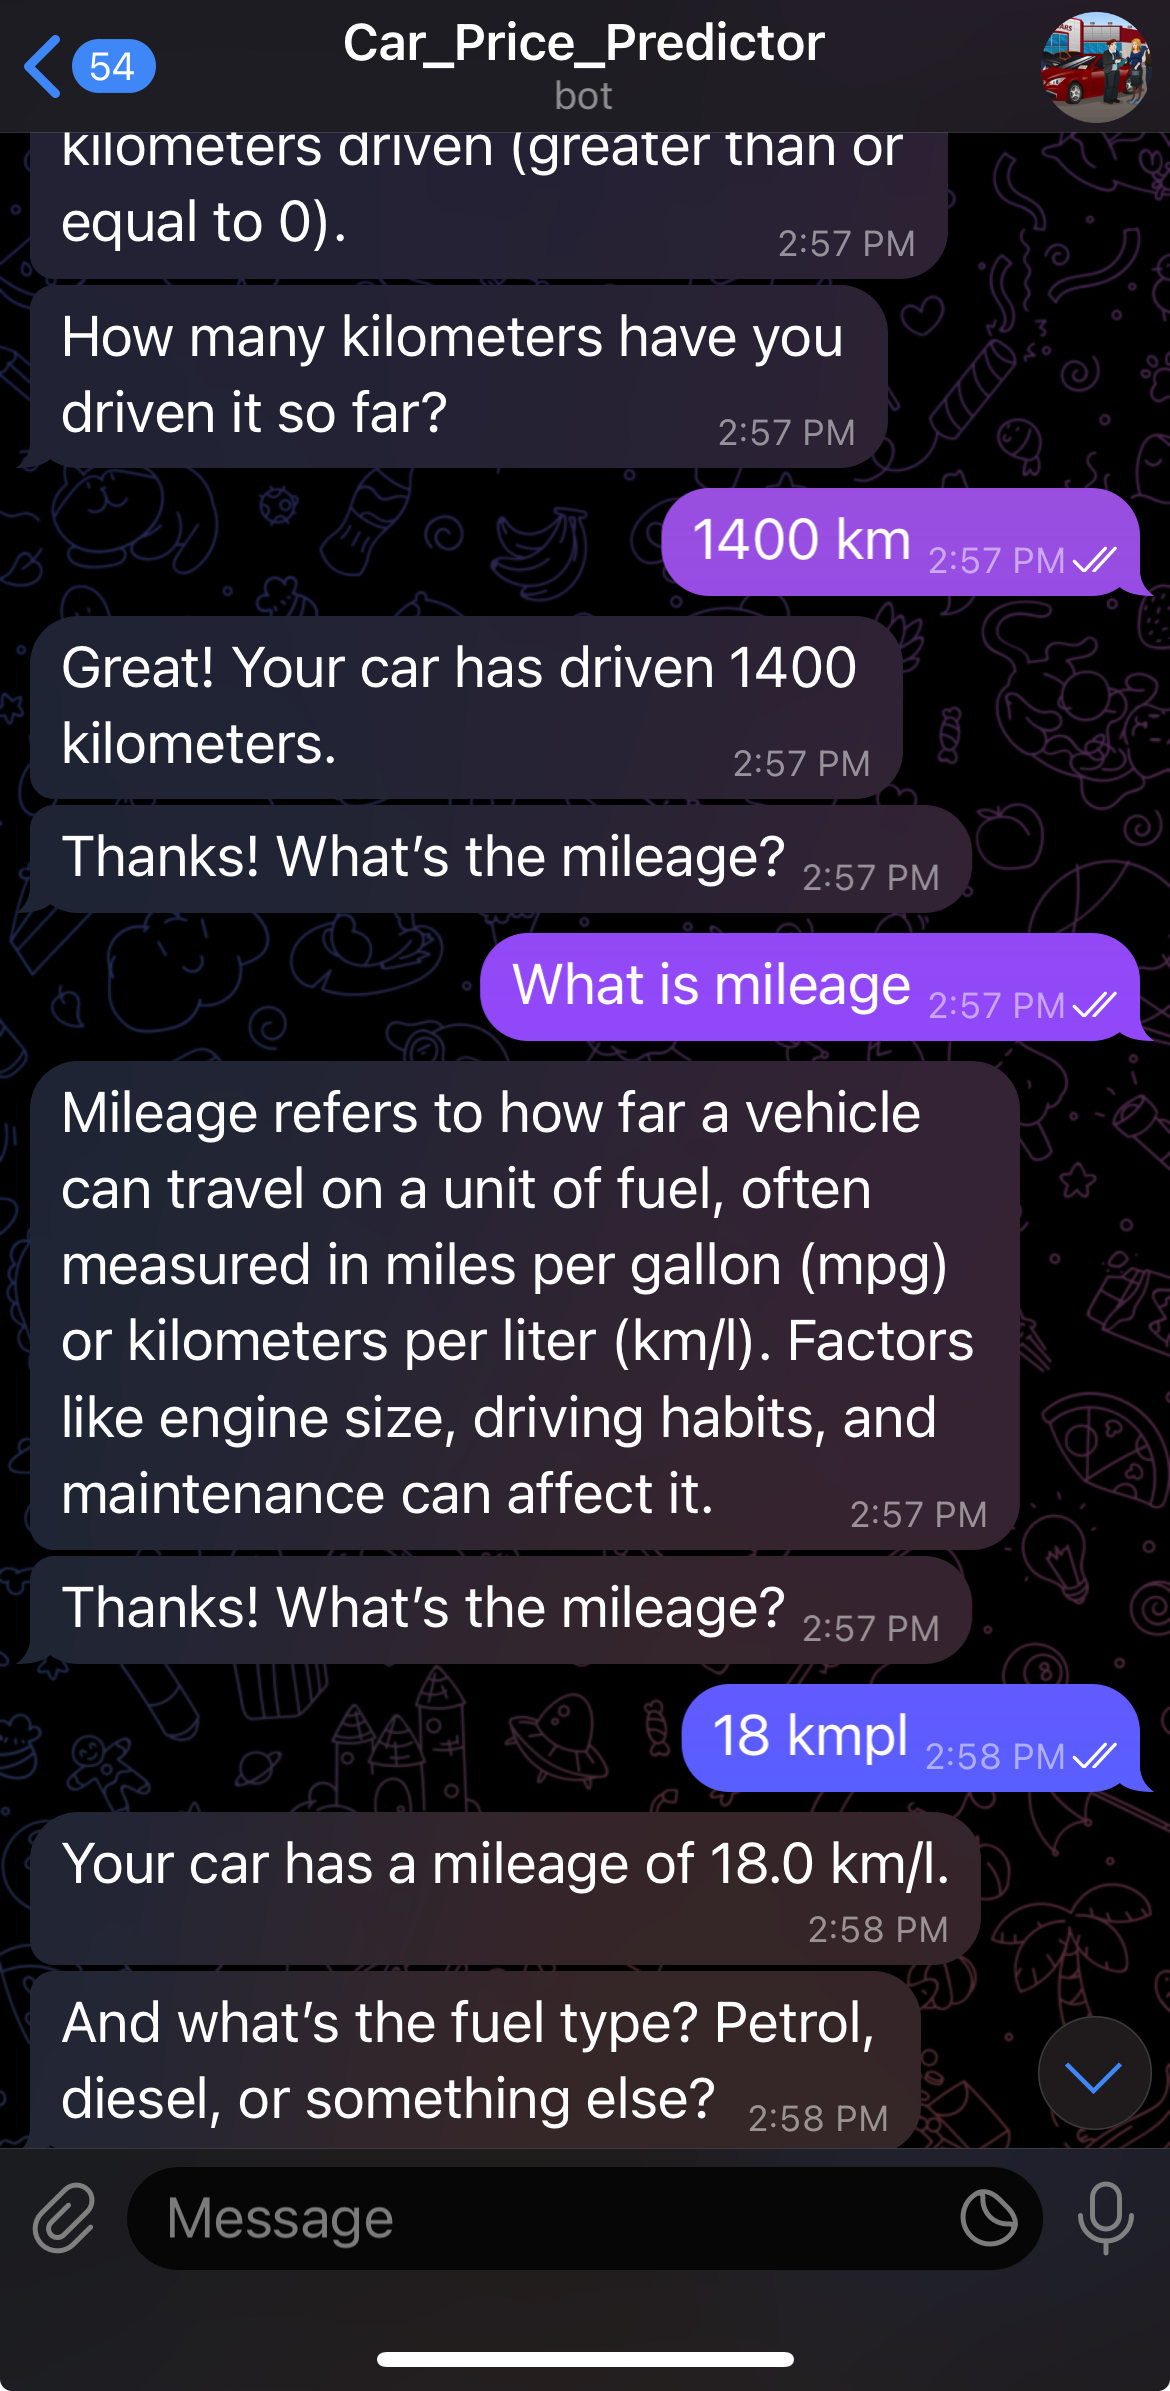
\includegraphics[width=0.8\textwidth]{2.jpg}
        \caption{Chat Flow Step 2: System provides feature explanation.}
        \label{fig:step2}
    \end{minipage}
\end{figure}

\end{frame}

\begin{frame}
\frametitle{Sample Chat Screenshots (Part 2)}

\begin{figure}[h!]
    \centering
    \begin{minipage}{0.45\textwidth}
        \centering
        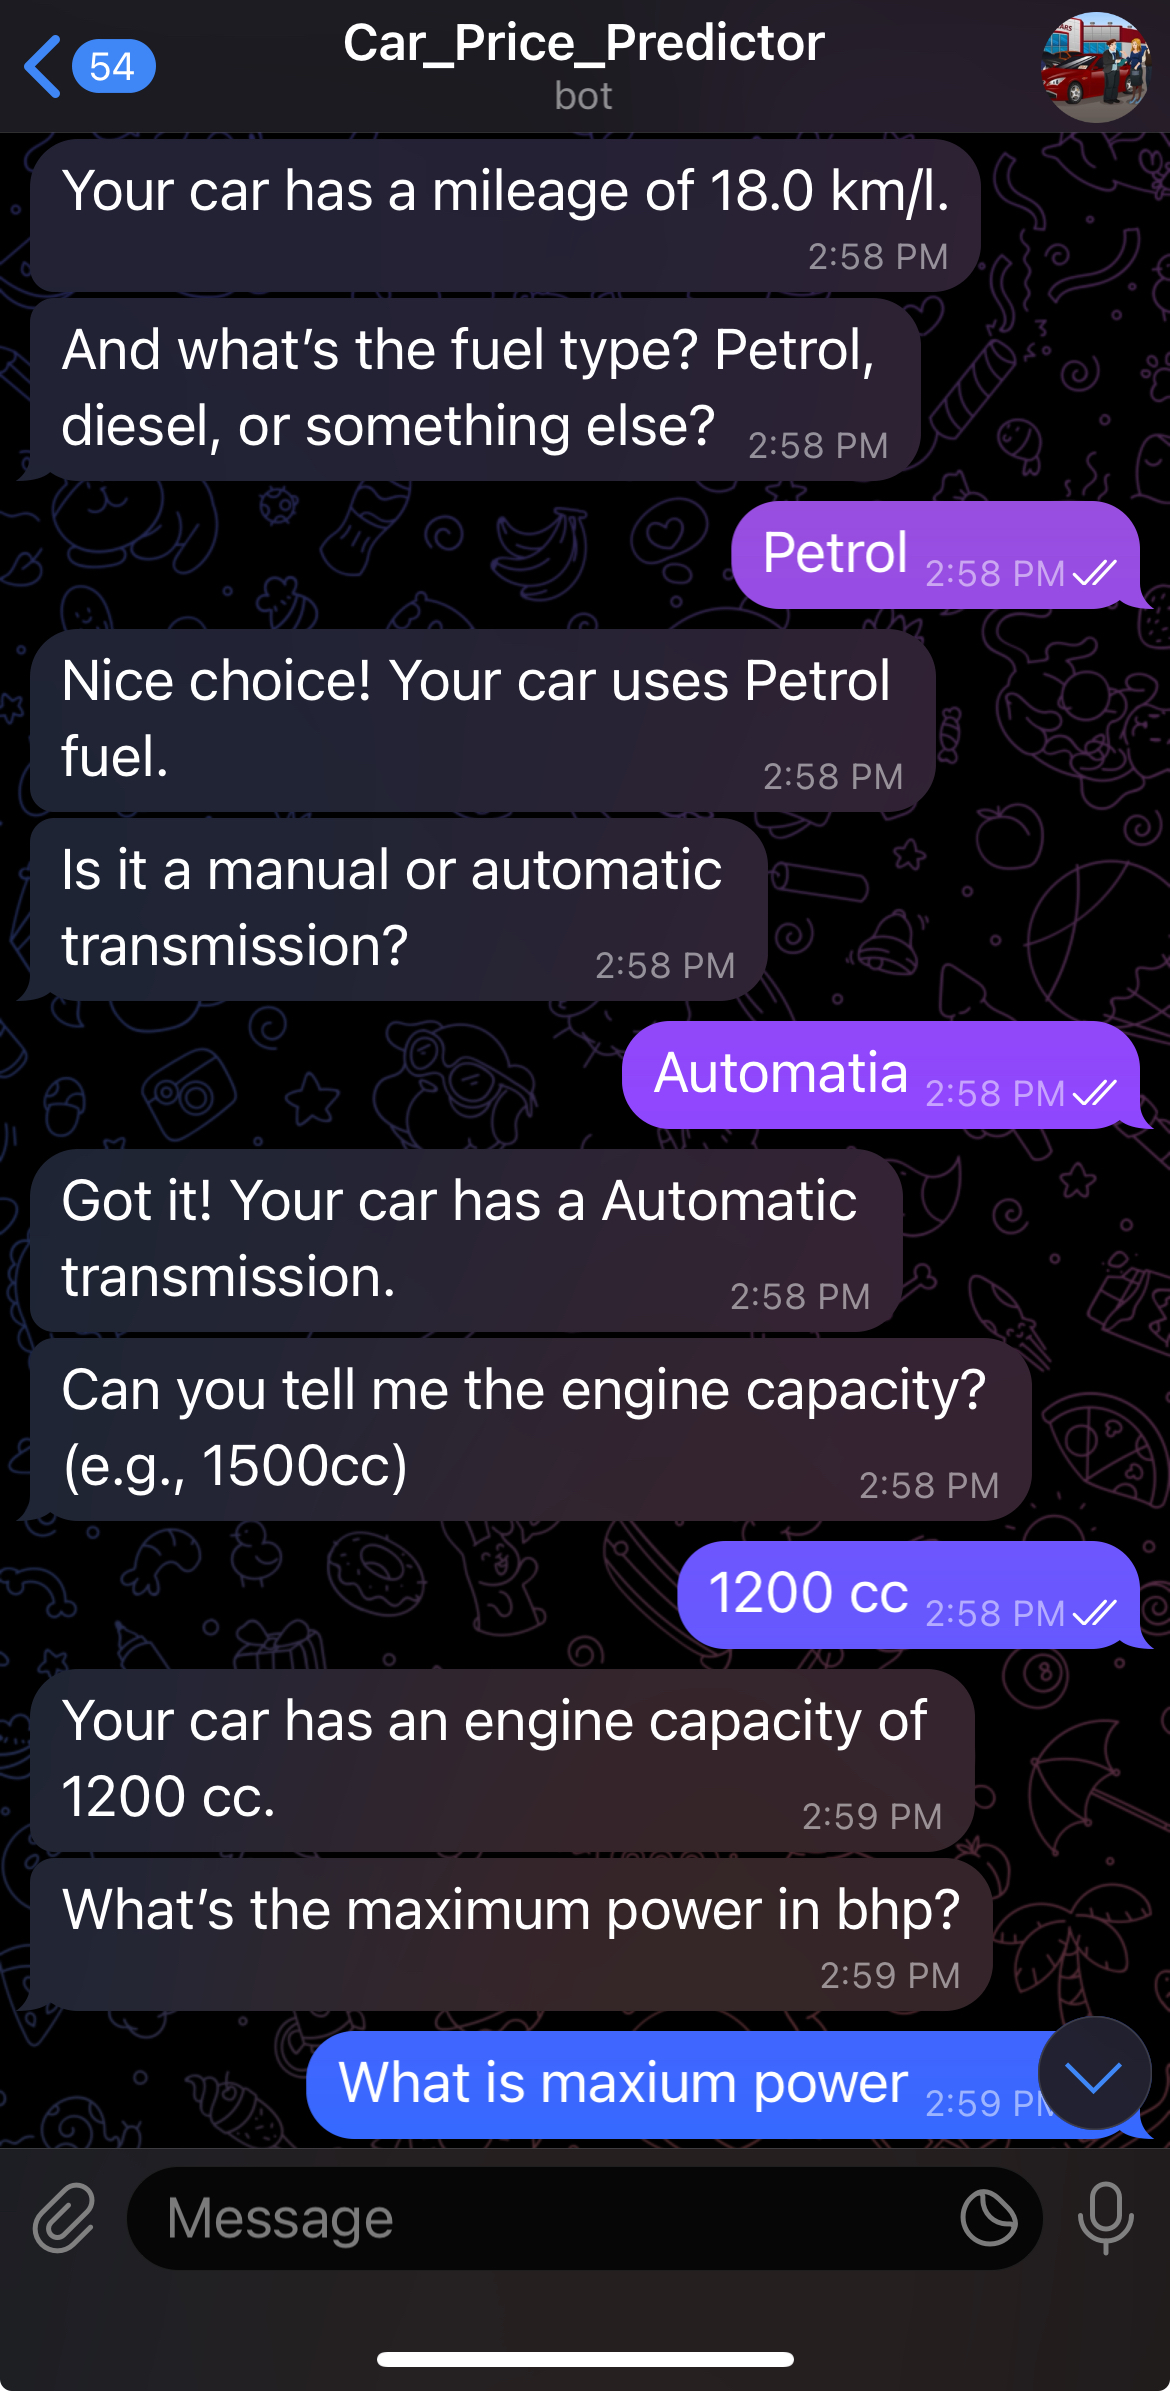
\includegraphics[width=0.8\textwidth]{3.jpg}
        \caption{Chat Flow Step 3: User provides feature values.}
        \label{fig:step3}
    \end{minipage}%
    \hspace{0.05\textwidth} % Add space between the images
    \begin{minipage}{0.45\textwidth}
        \centering
        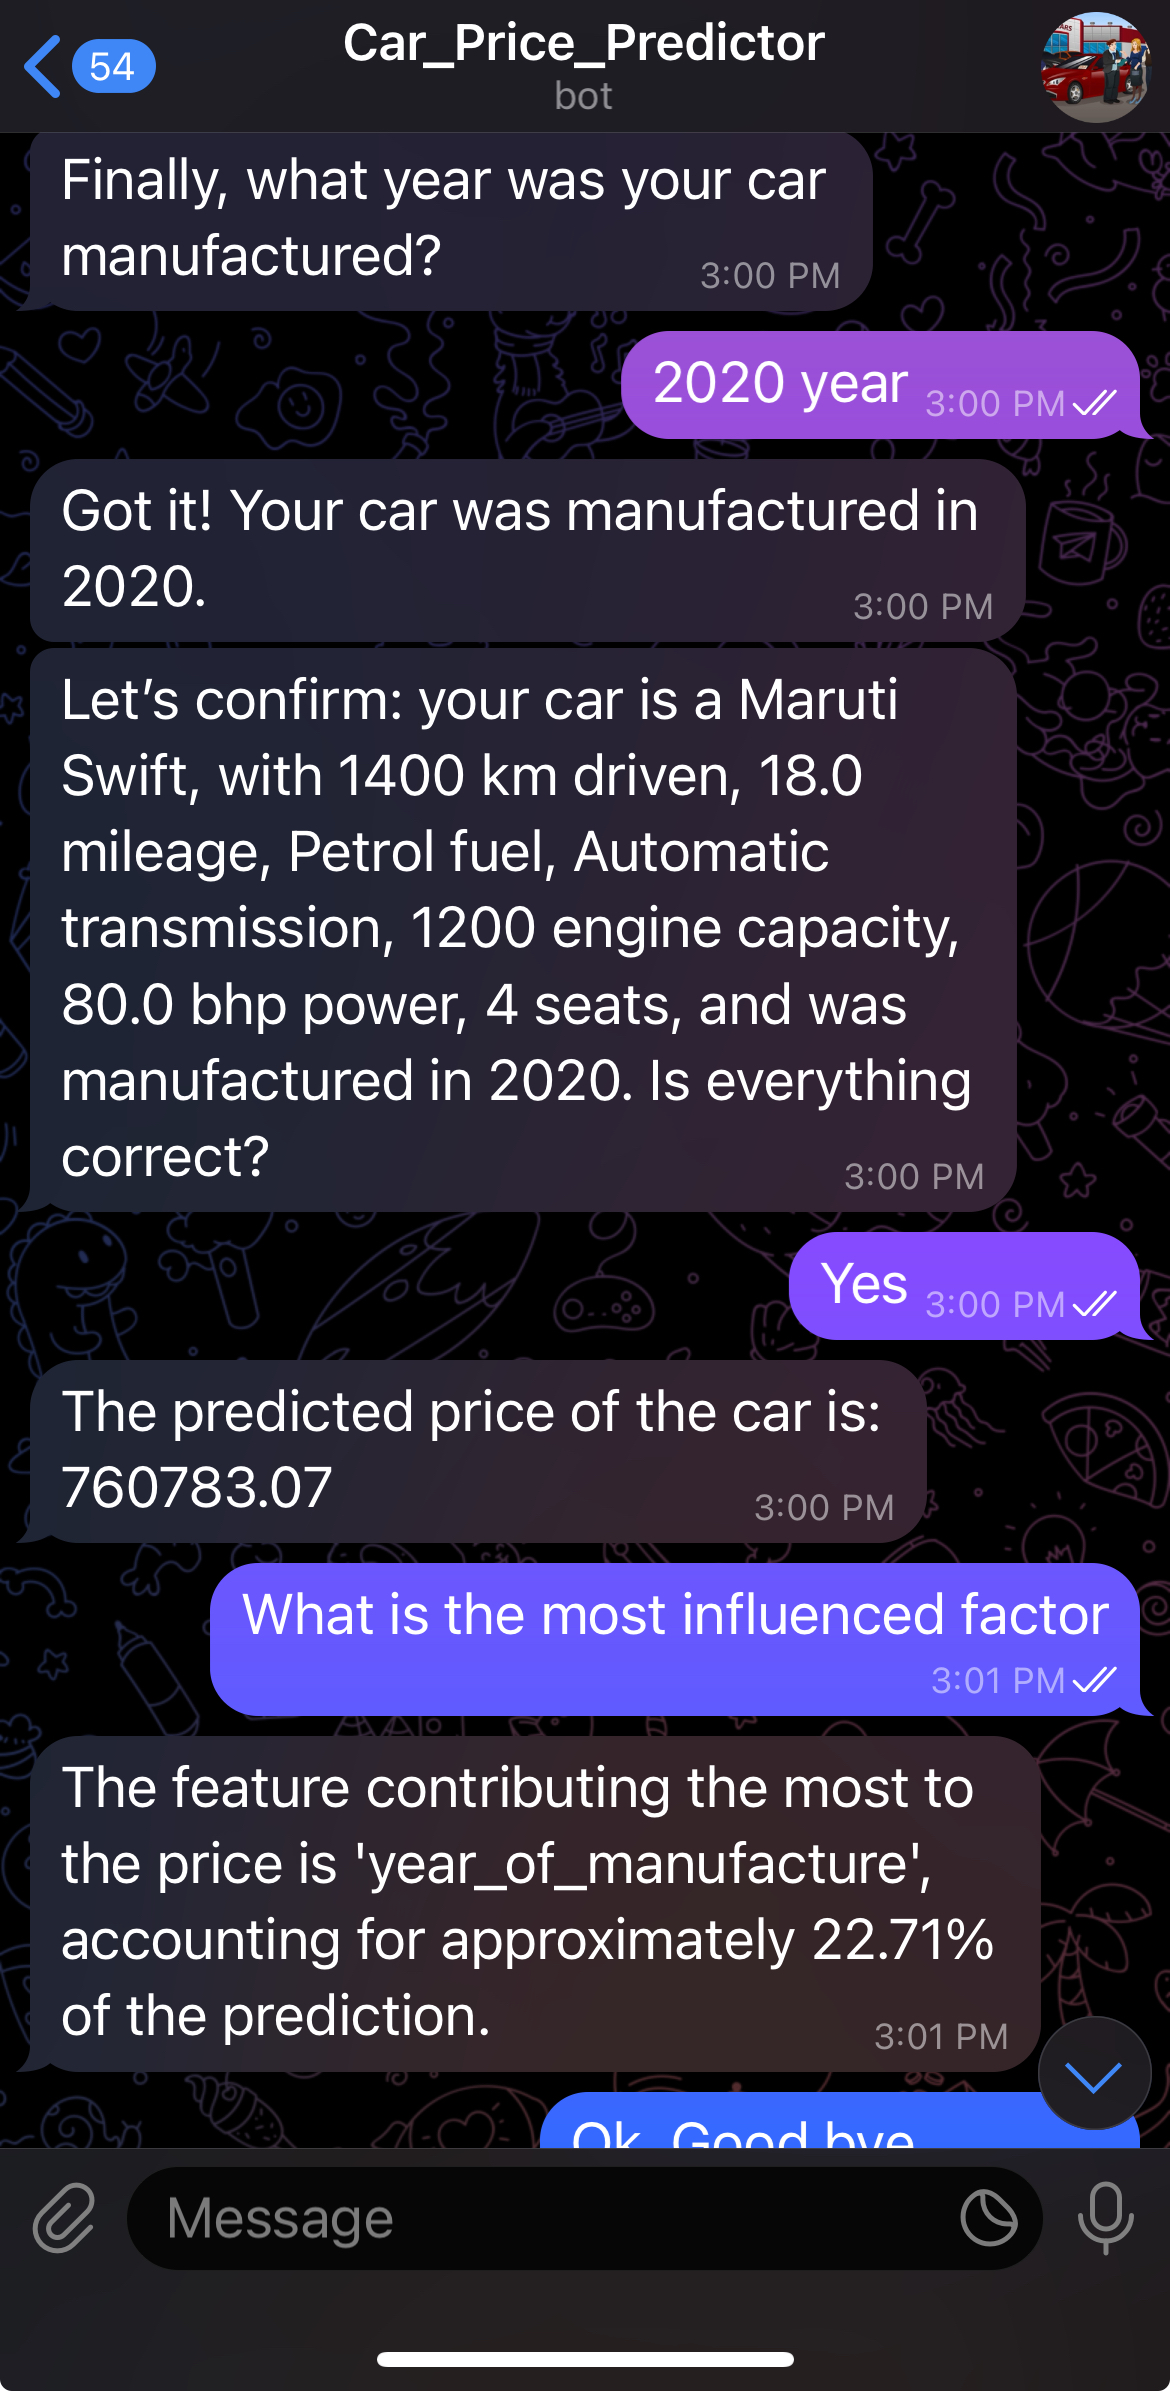
\includegraphics[width=0.8\textwidth]{4.jpg}
        \caption{Chat Flow Step 4: User receives car price prediction and SHAP explanation.}
        \label{fig:step4}
    \end{minipage}
\end{figure}

\end{frame}




\begin{frame}[t]{References}
\begin{thebibliography}{9}

\bibitem{rasa}
Rasa Technologies, ``Rasa Documentation,'' \textit{Rasa}, 2023. [Online]. Available: \texttt{https://rasa.com/docs/}
\bibitem{flask}
Armin Ronacher, ``Flask Documentation,'' \textit{Flask}, 2023. [Online]. Available: \texttt{https://flask.palletsprojects.com/}


\bibitem{shap-doc}
SHAP Documentation, ``SHAP (SHapley Additive exPlanations),'' 2023. [Online]. Available: \texttt{https://shap.readthedocs.io/en/latest/}

\bibitem{randomforest}
Leo Breiman, ``Random Forests,'' \textit{Machine Learning}, vol. 45, no. 1, 2001, pp. 5-32. [Online]. Available: \texttt{https://link.springer.com/article/10.1023/A:1010933404324}

\bibitem{randomforest-doc}
Scikit-learn, ``Random Forests,'' 2023. [Online]. Available: \texttt{https://scikit-learn.org/dev/modules/generated/\\sklearn.ensemble.RandomForestRegressor.html}



\end{thebibliography}
\end{frame}



\begin{frame}[t]{.}
    \centering
    \vspace{1cm}
    \textbf{\Huge{}}
    
    \vspace{0.5cm}
    \rule{0.5\textwidth}{0.5mm} % Horizontal line for design

    \vspace{1cm}
    \textbf{\Large{Thank You!}}

    \vspace{0.5cm}
    \rule{0.5\textwidth}{0.5mm} % Another horizontal line for symmetry
\end{frame}


\end{document}
